%************************************************
\chapter{Results}\label{ch:results}
%************************************************

In this chapter, we present the major results from simulated tests on the Chicago crime data set. First, we find that the accuracy of \pp does not exceed a baseline heuristic in the top 5\% of cells predicted. Second, we find that \pp, as assessed by the measure discussed in the previous chapter, is not fairer than the baseline heuristic. Third, we find that the fairness modifications presented in the previous chapter can work decently well at improving fairness while preserving the accuracy of \pp. Taken together, these results show that the benefits of \pp are overstated. We discuss this possibility as well as other implications in the next chapter.

\section{Accuracy}
\autoref{fig:accuracy} shows the accuracy of \pp compared to completely random prediction and the baseline measure, "naive counting." The baseline measure is comparable to a naive Bayes approach to predictive policing: rank each grid cell by the number of crimes that have taken place in that location over the whole observed dataset. In the language of \citet{mohler_marked_2014}, the naive counting measure corresponds to the "chronic hotspots" method with no decay in time (observations further back in time are weighted equally as more recent ones).
\begin{figure}[bth]
    \myfloatalign
    \subfloat[Overall, \pp predicts well...]
    {\label{fig:accuracy_overall}%
        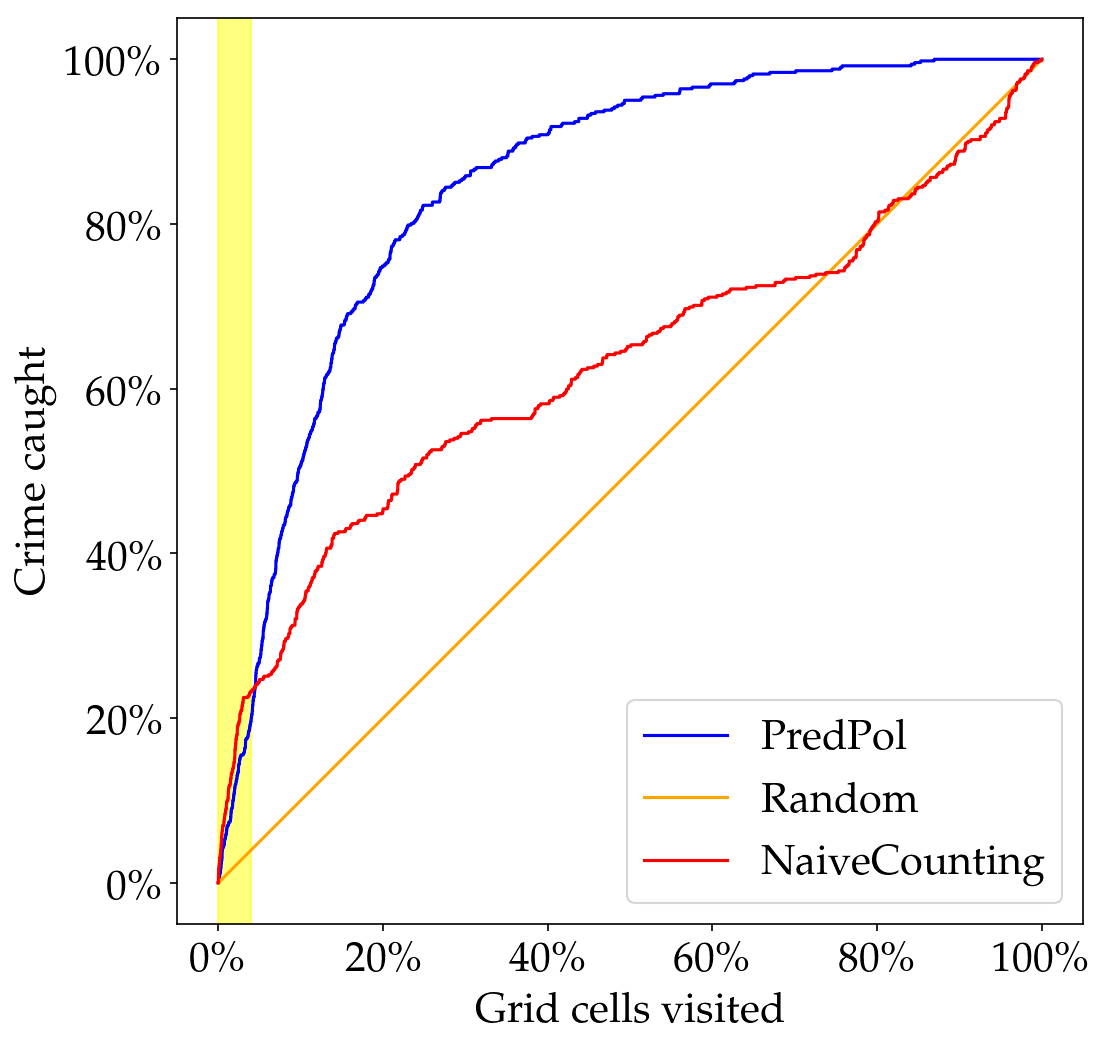
\includegraphics[width=.36\linewidth]{gfx/AccuracyAll.png}} \quad
    \subfloat[...but not in the top 5\% of grid cells.]
    {\label{fig:accuracy_zoom}%
        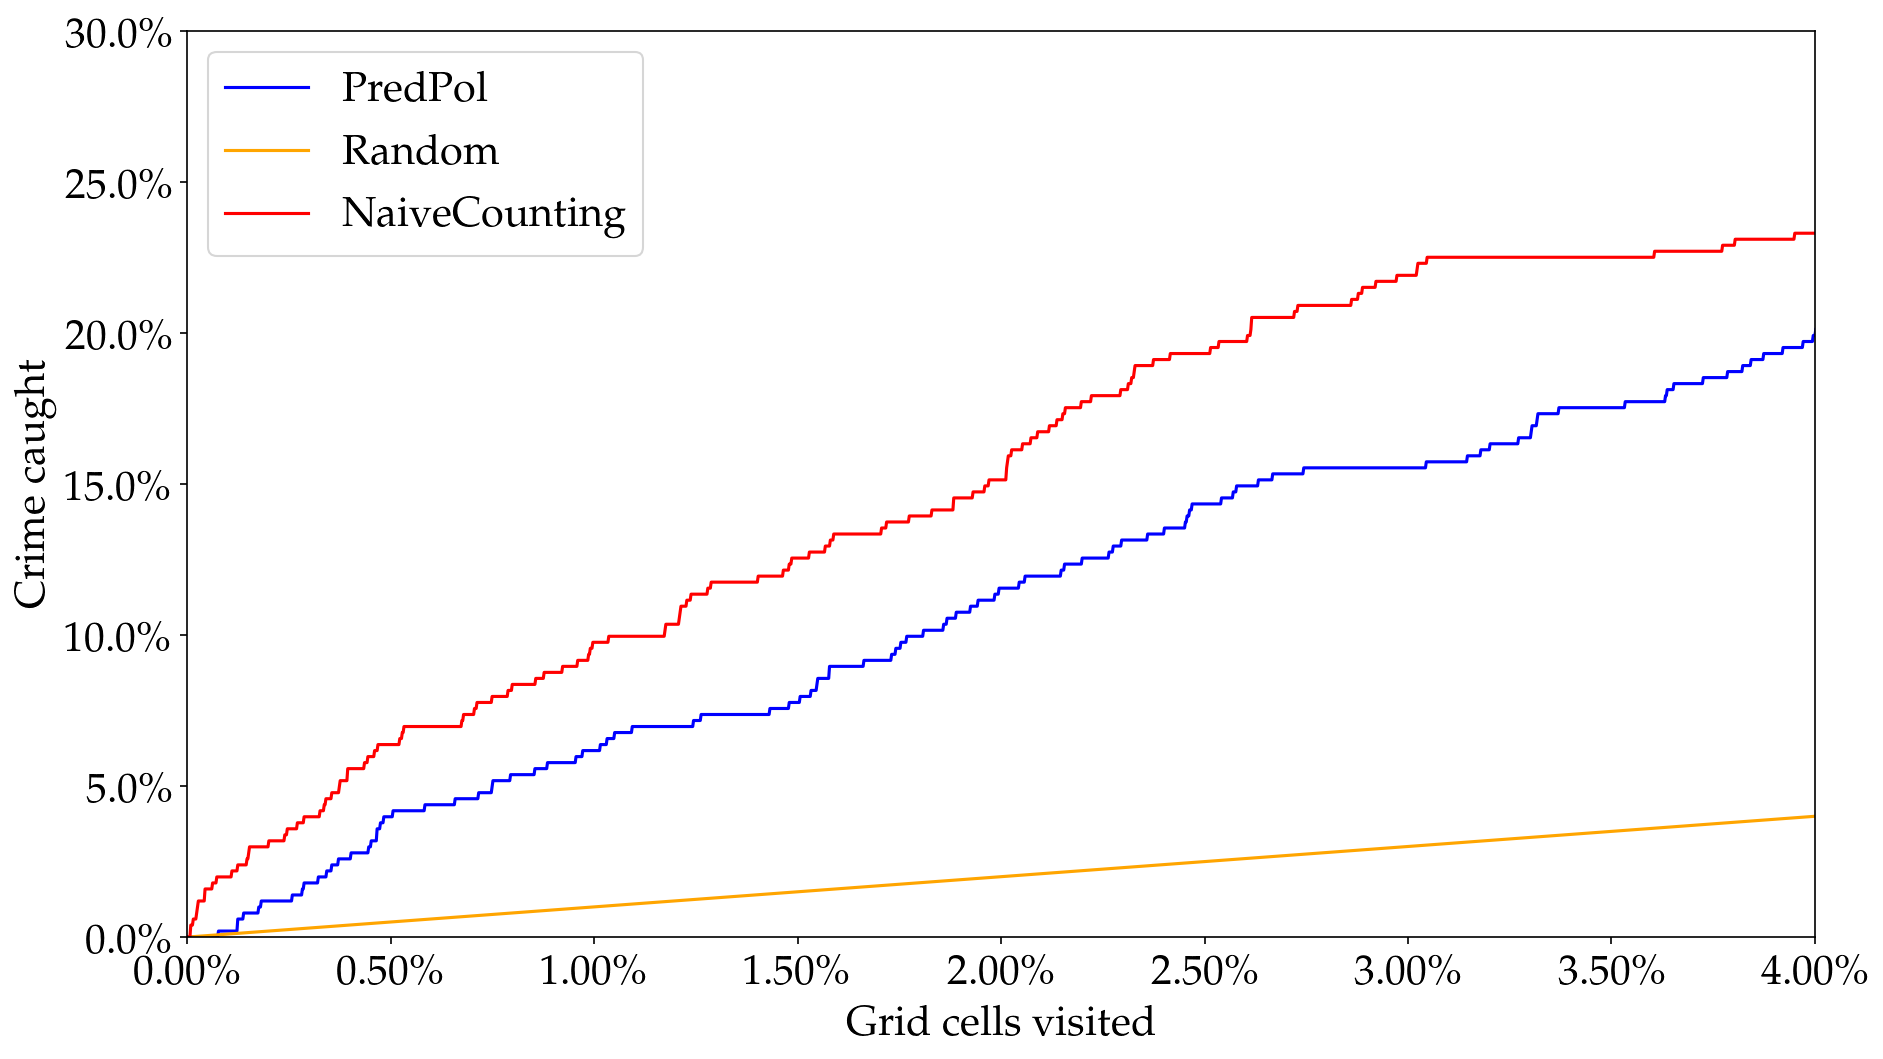
\includegraphics[width=.6\textwidth]{gfx/AccuracyZoom.png}} \\
    \caption[Accuracy curves comparing \pp and other baselines]{Accuracy curves comparing \pp and other baselines}\label{fig:accuracy}
\end{figure}
The results are shown as a function of the number of grid cells visited, since visiting more grid cells will tend to improve accuracy in general (these curves are similar to ROC curves in binary classification). The y-axis plots the percentage of crime caught, or the number of crimes that occur in the cells predicted as a percentage of the total crime occuring that day. Each curve is an average over 365 days of prediction in 2015.

Imagining that one had access to a perfect oracle, which knew in advance where each crime would occur, the results from such an oracle would plot a nearly perfect right angle at the upper left of \autoref{fig:accuracy_overall}. This reflects the fact that tiny percentage of grid cells each day are responsible for crime; knowing those locations in advance means that all of the crime occurring in a day could be captured by visiting just a few locations.

\pp shows increased accuracy when considered over the whole range of grid cells. The naive counting measure breaks down at around 80\% of grid cells predicted, when its performance becomes no better than randomly guessing.

However, visiting even 10\% of the grid cells on a map is unreasonable for police departments to accomplish. \citet{mohler_marked_2014} states that "a range of 250–500 150m $\times$ 150m cells is a realistic number for a city the size of Chicago," which correspond on the above plots to a range of $0.5\%$ to $1\%$ of grid cells.

\section{Fairness}
\autoref{fig:fairness} assesses the fairness of the same measures discussed in the previous section. Again, the x-axis is the percentage of grid cells visited/used by the algorithm. The y-axis computes the percentage of black crime captured (by the x\% grid cells predicted by the algorithm) minus the percentage of white crime captured (by the x\% grid cells predicted by the algorithm). When all grid cells have been predicted, 100\% of crime of both races has been captured, so each of the curves in figure~\ref{fig:fairness_overall} meet at $(1.0, 0.0)$.

A completely fair algorithm, by this metric, would lie directly on the x-axis. Random prediction has this property (noise in the curve is due to the random variation, and on different runs, the shape of the curve changes completely). It is interesting to note that random prediction is fair with regard to equalized odds while at the same time qualifying as a "fair through unawareness" classifier. Of course, random predictions' accuracy leaves much to be desired. Perfect prediction also lies on the x-axis, since perfect prediction captures all crime nearly instantaneously, thus also capturing equal percentages of both race's crimes. Curves above the x-axis indicate some amount of bias against blacks, while curves below the x-axis indicate some amount of bias against whites. However, because of how we operationalized race and fairness in \autoref{ch:fairpol}, one could easily draw the opposite conclusions: capturing a larger percentage of crime in black districts \emph{favors} blacks, and vice versa. We remain open to this alternative interpretation. The point is to try and achieve equality for both races.

\begin{figure}[bth]
    \myfloatalign
    \subfloat[\pp is slightly fairer over all cells...]
    {\label{fig:fairness_overall}%
        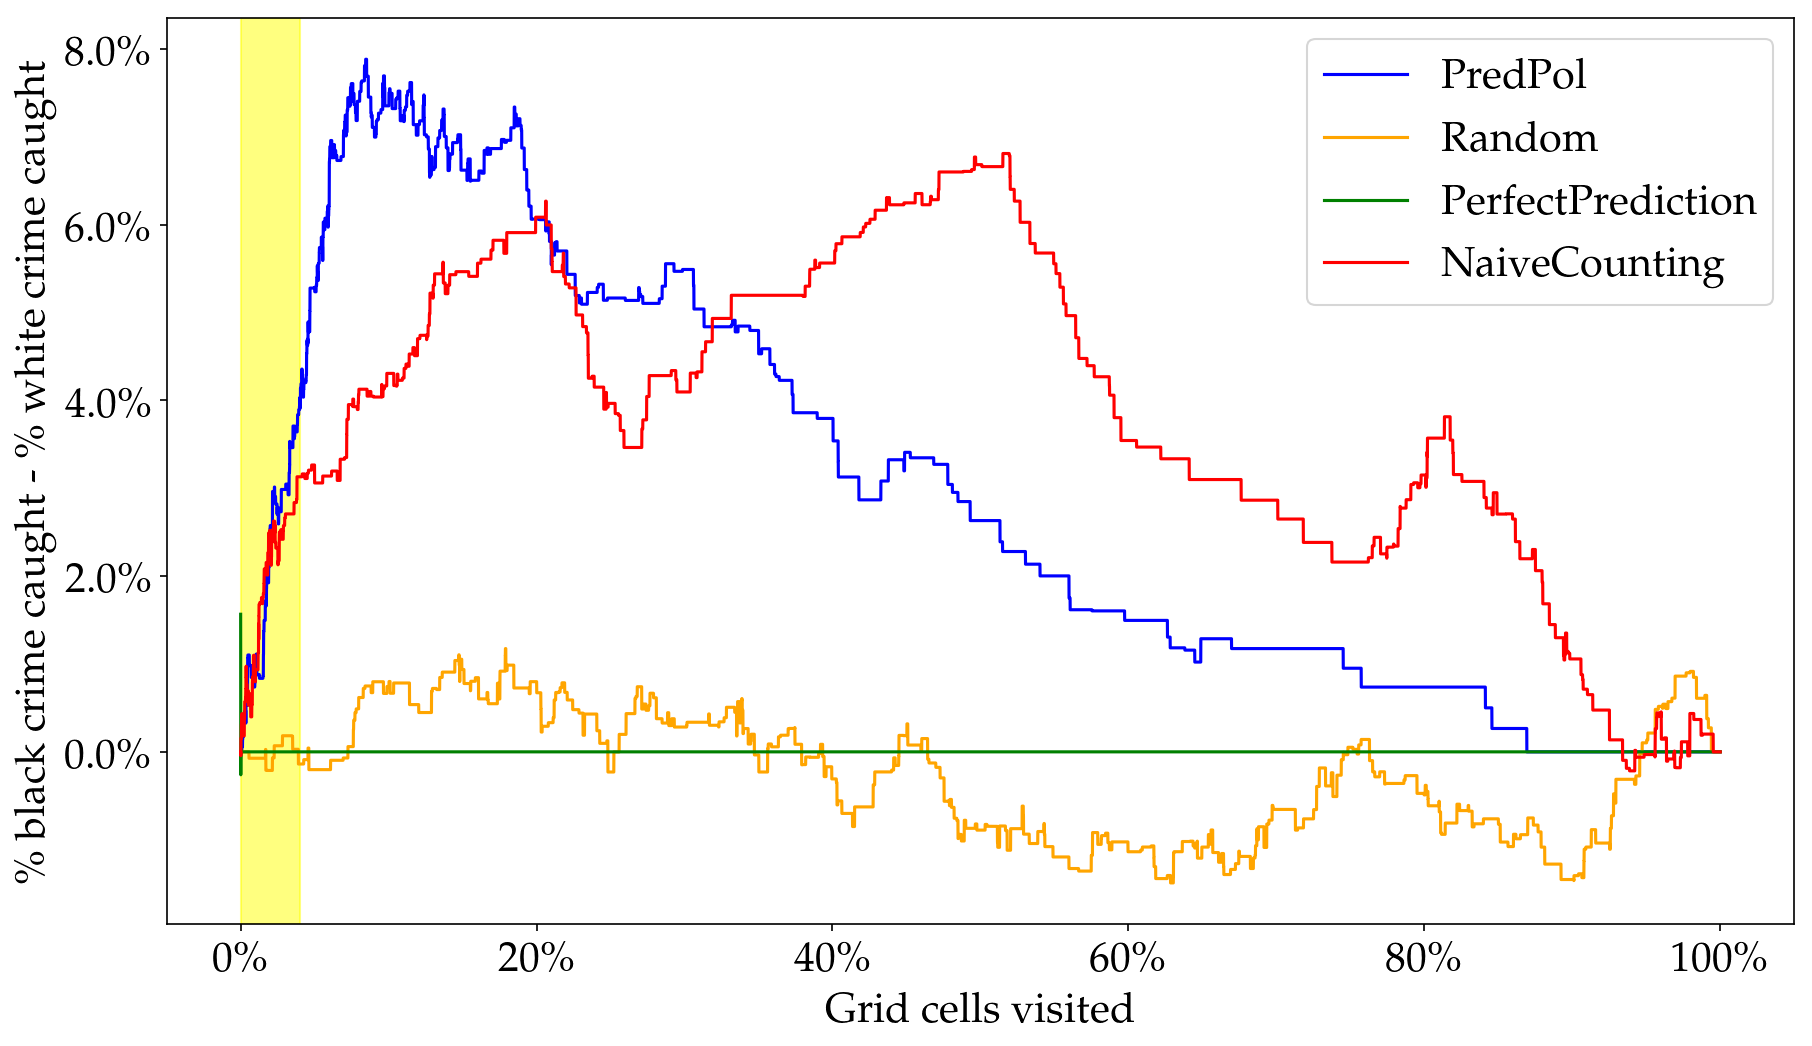
\includegraphics[width=.6\linewidth]{gfx/FairnessAll.png}} \\
    \subfloat[...but not especially so in the top 5\% of grid cells.]
    {\label{fig:fairness_zoom}%
        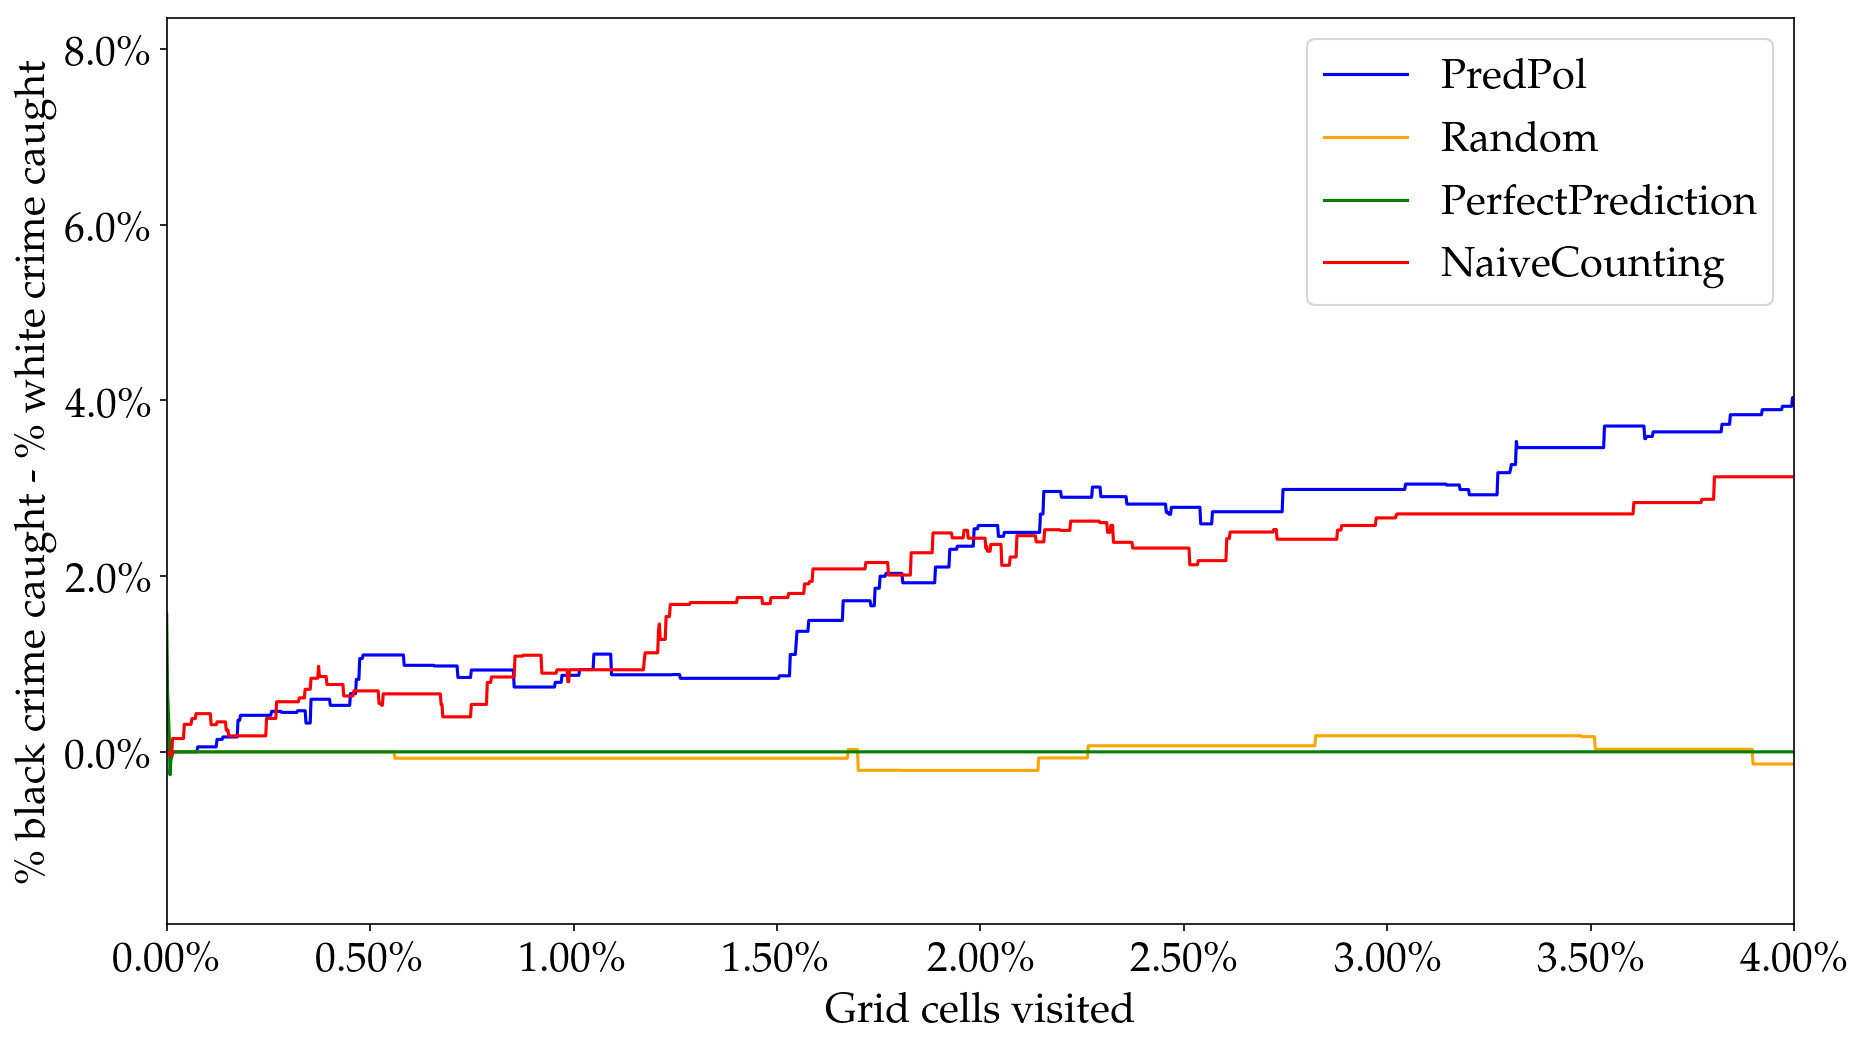
\includegraphics[width=.6\textwidth]{gfx/FairnessZoom.png}} \\
    \caption[Fairness curves comparing \pp and other baselines]{Fairness curves comparing \pp and other baselines}\label{fig:fairness}
\end{figure}

The differences between \pp and the baseline measure are less apparent on fairness. In the range of cells discussed in the previous section, \pp hews closer to the x-axis than the baseline measure.

One interesting aspect is that the fairness curves for both \pp and naive counting never go below the x-axis; in other words, both measures always capture a larger percentage of black crime than white crime. We suggest possible reasons for this in \autoref{sec:discussion}.

\section{Fairness Modification}
\begin{figure}[bth]
    \myfloatalign
    \subfloat[The modification has comparable accuracy...]
    {\label{fig:mkp_accuracy}%
        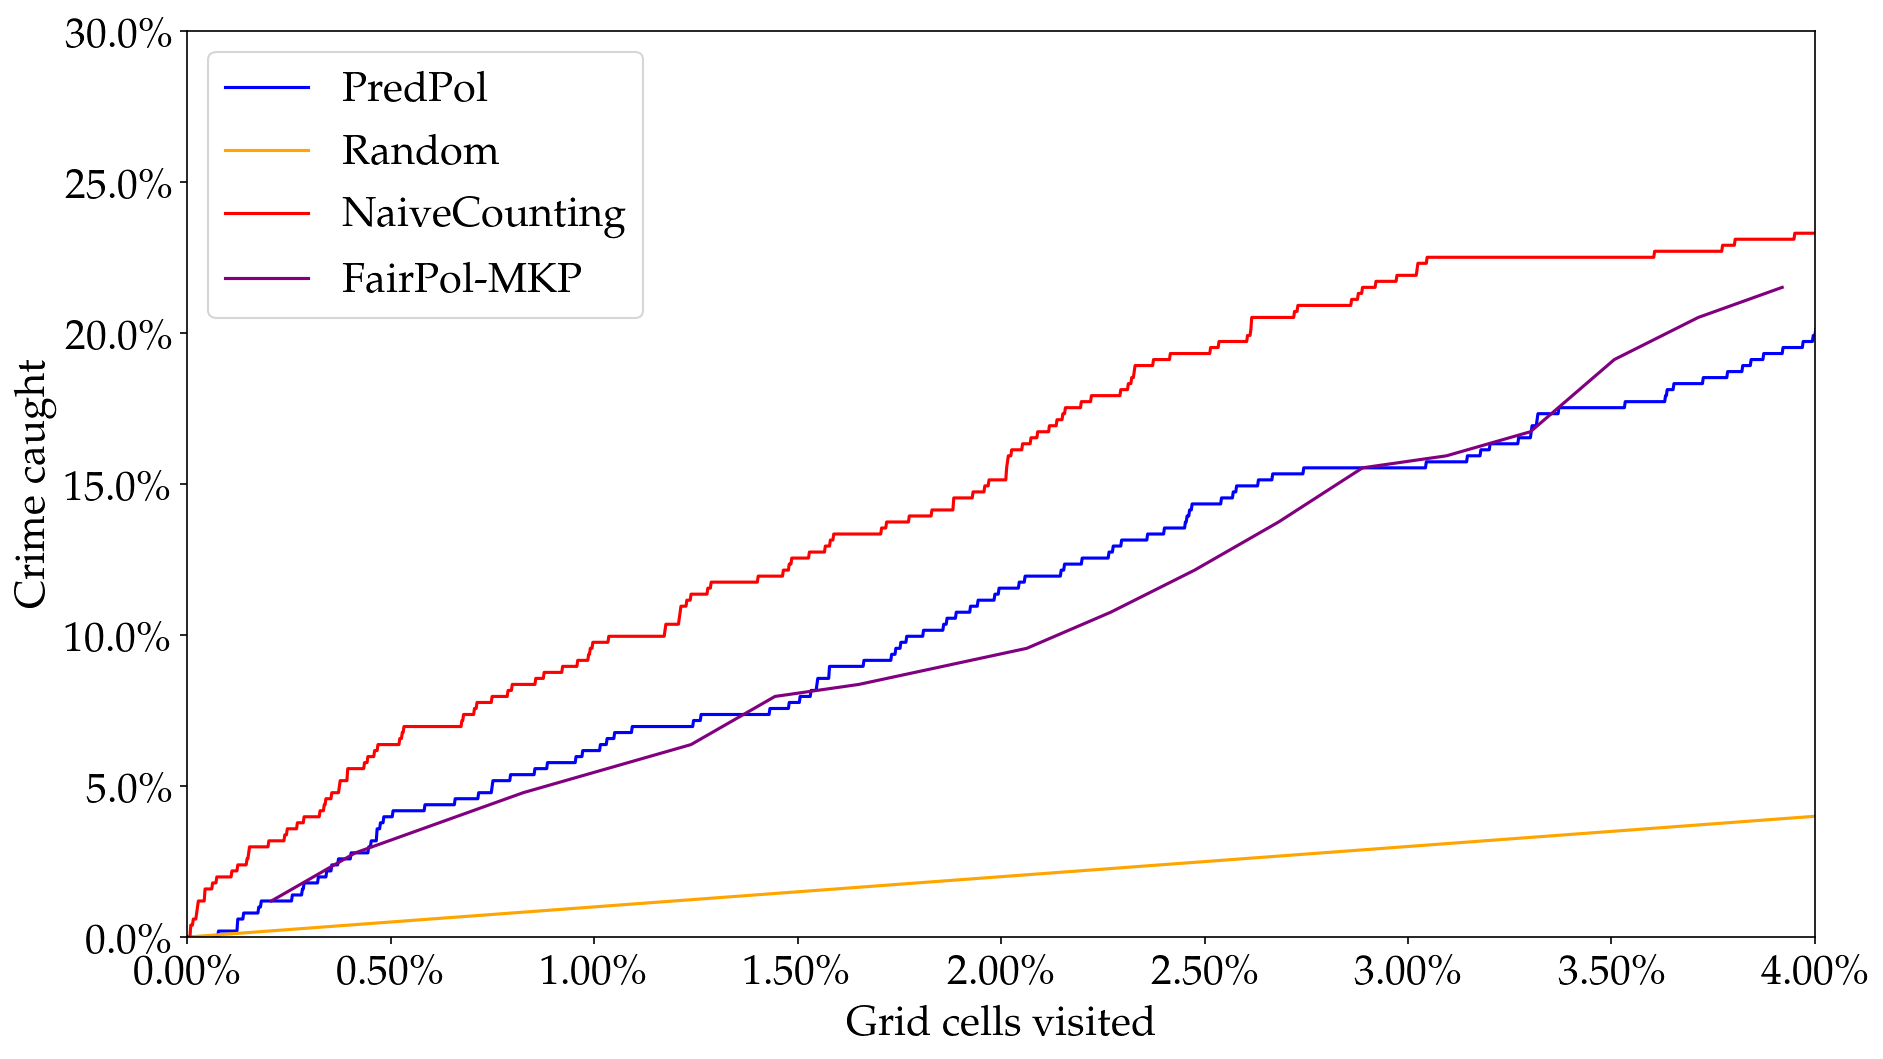
\includegraphics[width=.6\linewidth]{gfx/MKPAccuracy.png}} \\
    \subfloat[...while being significantly fairer.]
    {\label{fig:mkp_fairness}%
        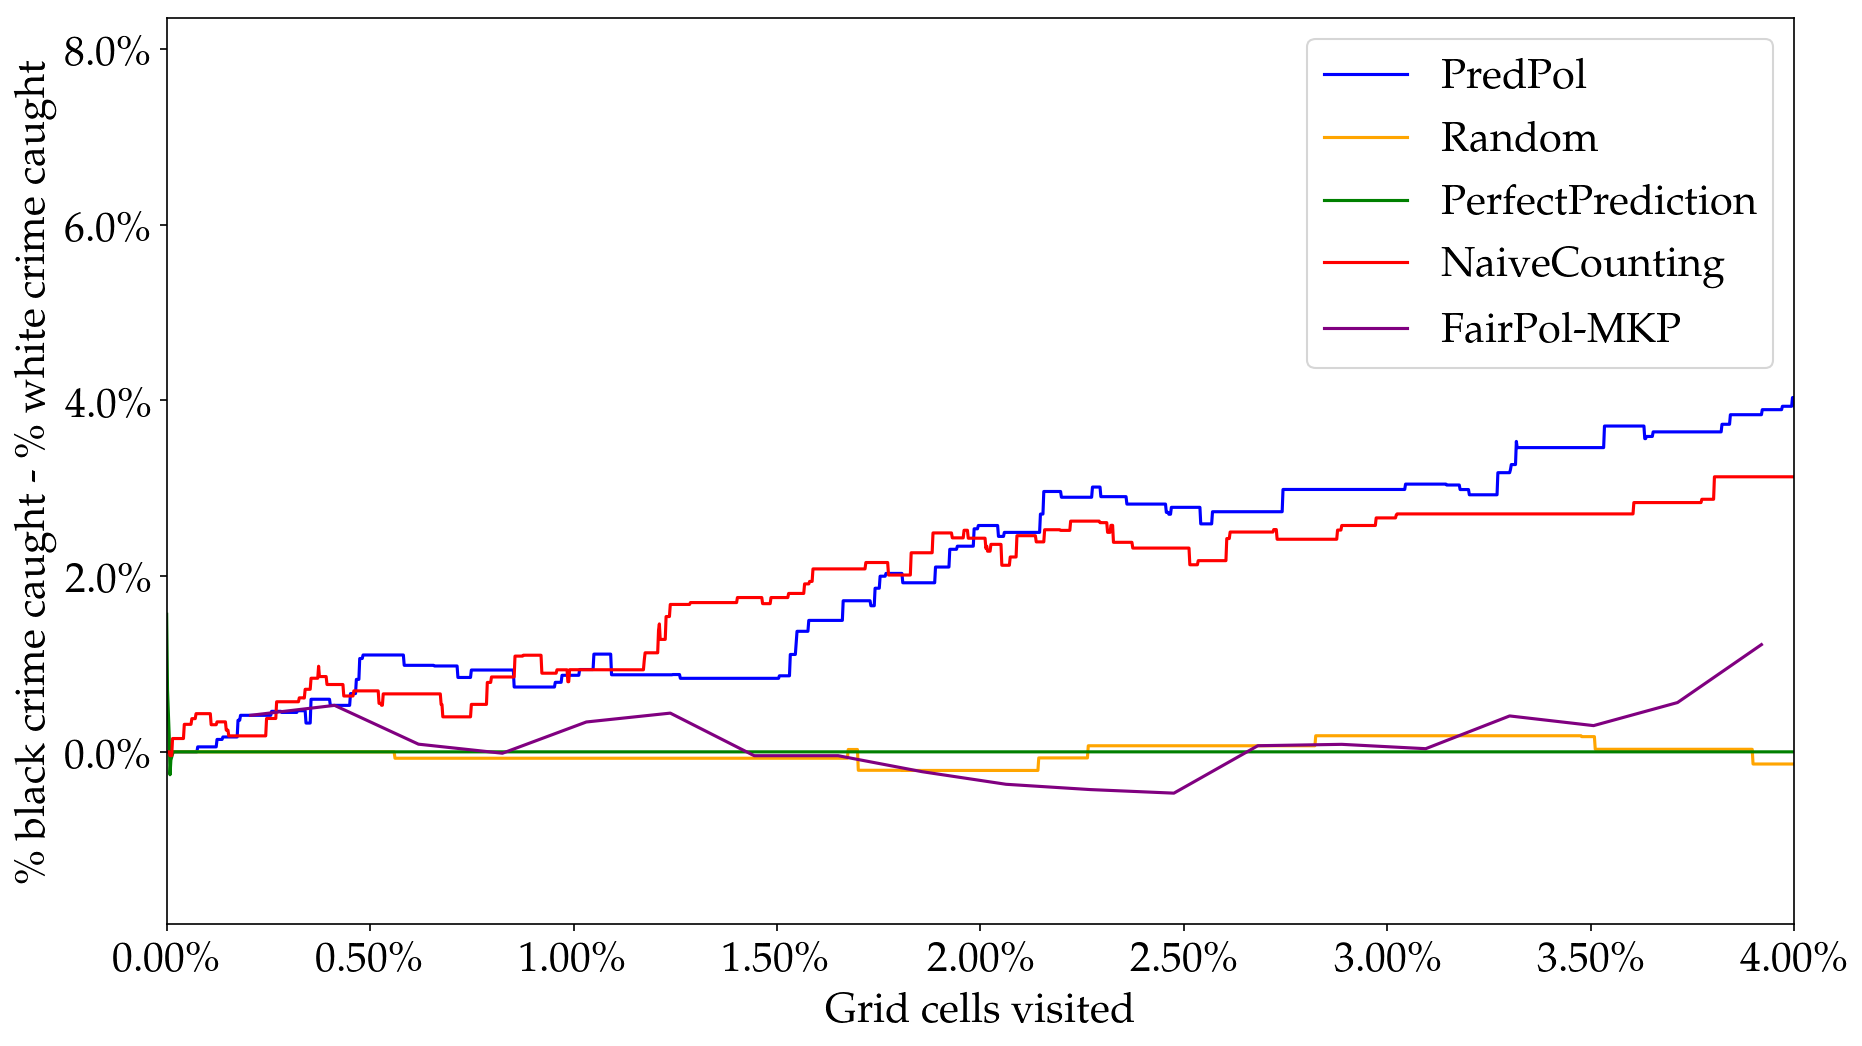
\includegraphics[width=.6\textwidth]{gfx/MKPFairness.png}} \\
    \caption[The accuracy and fairness of the post-processing modification]{The accuracy and fairness of the post-processing modification (purple) ($D = 1.25\%$)}\label{fig:mkp}
\end{figure}
Finally, \autoref{fig:mkp} shows the result of the post-processing task suggested in \autoref{ch:fairpol}. By seeking combinations of grid cells that together constitute fairer policing, these results show that achieving fairer prediction without comparable hits to accuracy is possible.

% TODO: Table: Numerical Summary of Results
% TODO: Translate the percentage differences into real-victimization (number of lives lost, affected)

\section{Caveats} \label{sec:caveats}

Before proceeding to a full discussion of the results, we would like to, in the interest of transparency and future research, highlight several limitations of the present research. The most important omission is the lack of using different types of crime to predict one another, as done in \citet{mohler_marked_2014}. That model uses the historical record of, say, burglaries, to assess increased likelihood of say, homicides. One direction for future research is to implement the full model described in \citet{mohler_marked_2014} and attempt to replicate the results of this research. Creating a plausible baseline method for this kind of prediction is complicated by the fact that different types of crime occur at very different rates than others; a naive Bayes method that treats all crime equally would be dominated by the most prevalent crime type.

Nevertheless, it still seems plausible that a baseline measure, such as the chronic hotspots method discussed in \citet{mohler_marked_2014} and similar to the naive counting measure used here, could achieve comparable performance to \pp. In several places throughout the text, \citet{mohler_marked_2014} also acknowledges that chronic hotspots account for most of the crime in the dataset. If this is indeed the case, then the discussion of ethics in the following section is still likely to hold merit. 

% Manual inspection of the figures in \citep{mohler_marked_2014} still suggest that the naive counting approach is comparable to the full marked point processes approach.

There are a few smaller differences that may have led to a difference in findings in the present research and \citet{mohler_marked_2014}. First, the number of grid cells in our simulation seems to differ than that in \citet{mohler_marked_2014}. It seems that Mohler examined a smaller geographical region than in the present research, but Mohler did not make note of this detail in their paper. Second, the Chicago dataset is known to change over time as the agency responsible for marinating the data re-randomizes the locations of crimes in order to protect privacy.

Finally, there may have been errors in our simulation, for which we take full responsibility. A more detailed explanation of methods along with replication code is available in \autoref{app:methodology}.

\section{Discussion} \label{sec:discussion}

Barring the caveats mentioned in the previous section, it is unclear why \pp does worse than the naive counting measure in the region specified. We hypothesize, for further testing, that some amount of constructive interference may be occurring: in the middle zone between two crime hotspots, \pp predicts a high amount of crime, despite being exactly in the middle of where the crime would likely occur.

With regard to normative issues, \citet{mohler_marked_2014} state that their model results in a 17\% in accuracy from the measures they consider, and that, "[g]iven the high societal cost of homicide and serious gun crime (DeLisi et al., 2010), which is estimated to be billions of dollars a year in Chicago, even a few percent decrease in the homicide rate due to hotspot policing with a more accurate ranking method would be of significant societal benefit." Building off of the empirical results presented in this chapter, we posit that there may also be costs to fairness and transparency which should also be weighed against the benefits of predictive policing. If a simpler method for prediction (i.e. the hotspot policing approach) generates nearly as good accuracy in predictions, is more equitable across protected groups, and is easier to explain to the affected population, there are good reasons for preferring that simpler approach.
\begin{figure}[bth]
    \myfloatalign
    \subfloat[Black population as a percentage of total = black + white]
    {\label{fig:heatmap_black2}%
        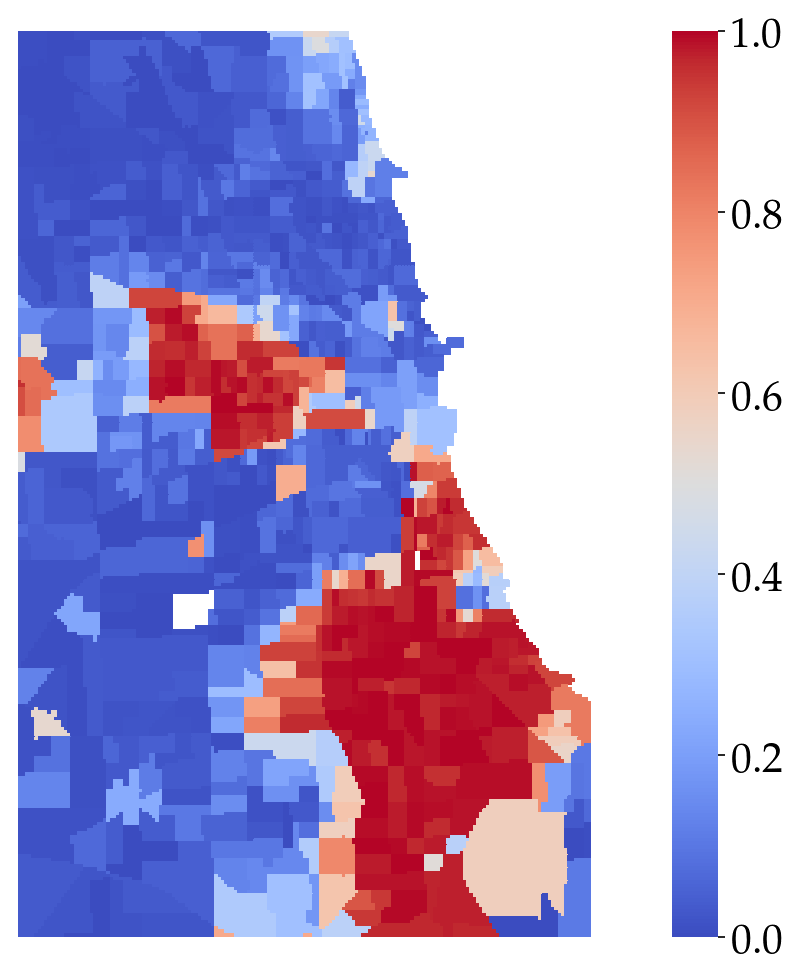
\includegraphics[height=.45\textheight]{gfx/HeatmapBlack.png}} \quad
    \subfloat[Number of actual crimes]
    {\label{fig:heatmap_actual}%
        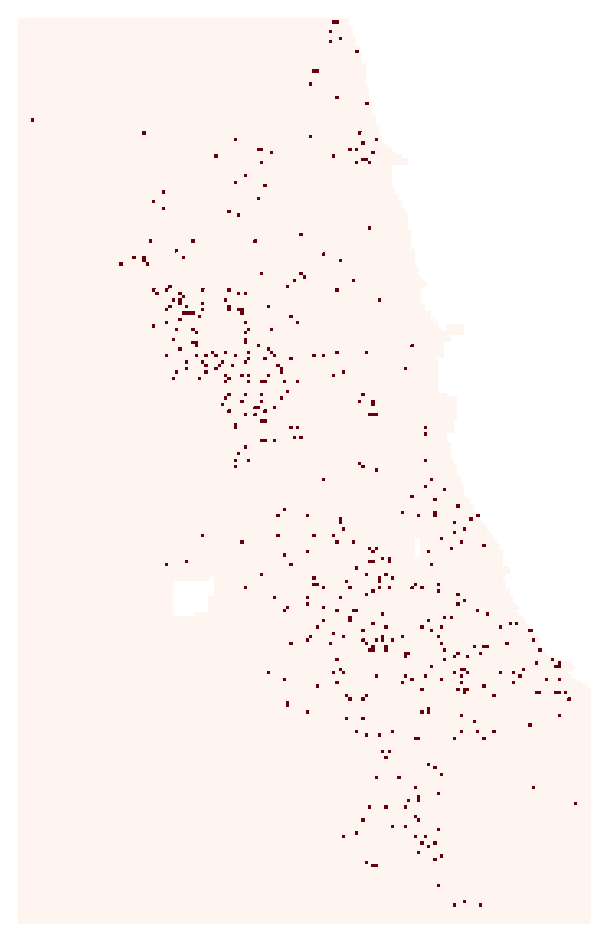
\includegraphics[height=.45\textheight]{gfx/HeatmapActual.png}} \\
    \caption{The visual relationship between race and actual number of crimes}
    \label{fig:actual}
\end{figure}

First, despite the success of machine learning in some areas, such as image recognition or playing games, algorithms in social applications have a much more difficult time achieving comparable success. The difficulty likely arises from the dearth of high-quality data and human understanding of the social phenomena that the algorithms interact with. Therefore, any purported accuracy benefits to a machine learning algorithm in a social application must be scrutinized carefully. It seems unlikely that we will see comparable improvements in accuracy in predictive policing as we have with, say, image or speech recognition.

Both \pp and naive counting police black crime more than white crime. We posit that this occurs because one group's crime is more concentrated in one area than another. \autoref{fig:heatmaps_f_hat} show the distribution of $\hat{f}$ values in the Chicago region while \autoref{fig:actual} shows the actual locations of crime. While there is a weak relationship between race and number of crimes (as stated previous, Pearson's r of 0.11), there are still a number of crimes in whiter areas in the northern region of the map. On the other hand, the crimes in blacker areas tends to be closer clustered together.

Because of its aftershock modeling, \pp would tend to exploit the clustering of black crime and predict those regions more frequently, even though a good predictor would also try and account for the sparser crime occurring in the north of the map. That explains how \pp is initially more unfair than naive counting (in the range of 0-30\% cells predicted) in \autoref{fig:fairness_overall}. Nevertheless, \autoref{fig:fairness_zoom} does show that this difference in fairness in negligible in the range of grid cells that a police department could actually visit.

\begin{figure}[bth]
    \myfloatalign
    \subfloat[Where crimes affecting black...]
    {\label{fig:heatmap_pct_black}%
        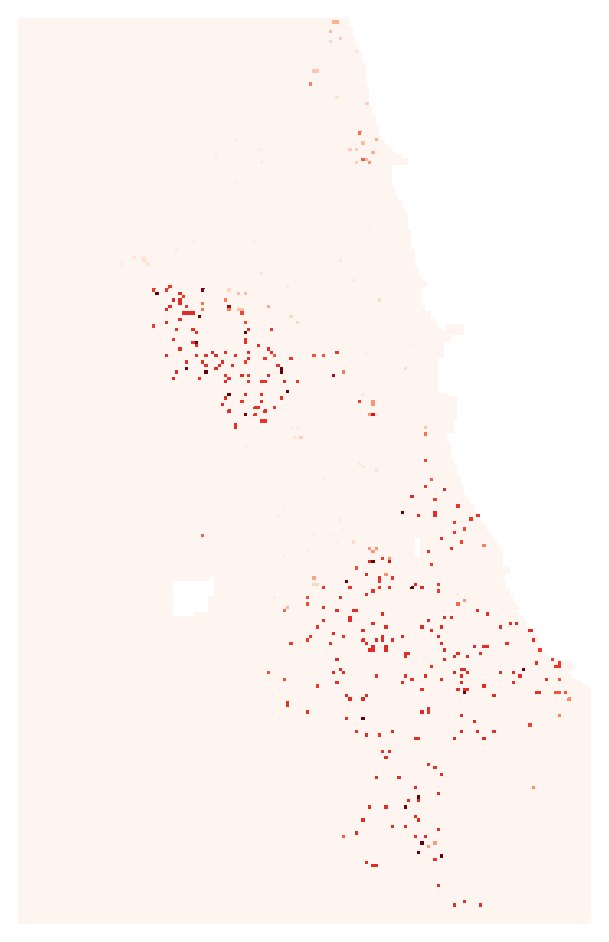
\includegraphics[width=.48\linewidth]{gfx/HeatmapPctBlackCrime.png}} \quad
    \subfloat[...and white people occur]
    {\label{fig:heatmap_pct_white}%
        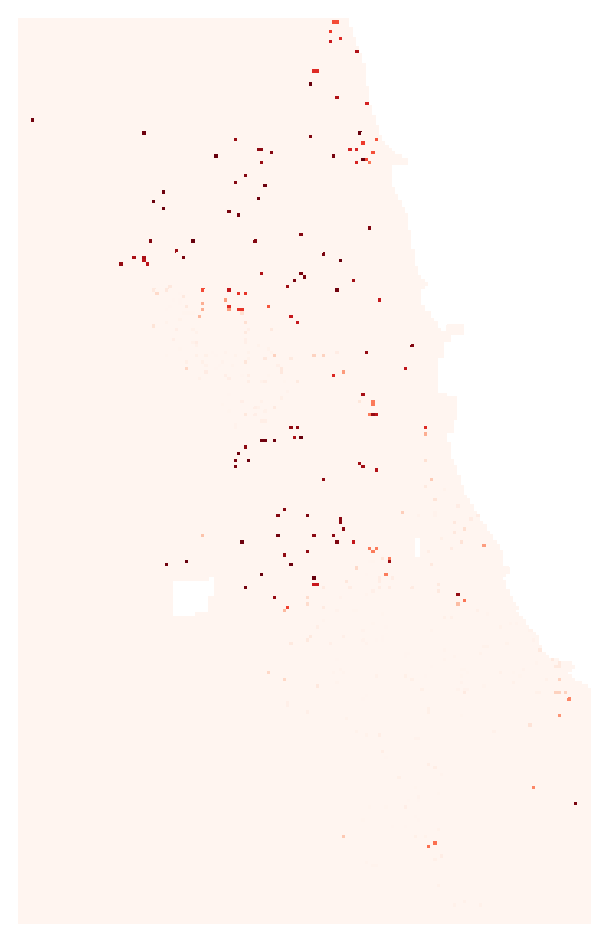
\includegraphics[width=.48\linewidth]{gfx/HeatmapPctWhiteCrime.png}} \\
    \caption{Heatmaps of $\hat{f}$ values}
    \label{fig:heatmaps_f_hat}
\end{figure}

Finally, \pp is likely to be less transparent to a policed community than a measure as simple as the naive counting measure. Patrol officers and officials are not likely to understand how and and why the model generated its results, since the product is sold to police departments as a black box. Moreover, relying on a third-party vendor to handle predictions runs the risks of feedback loops suggested by other researchers \citep{lum_predict_2016,ensign_runaway_2017,ensign_decision_2018}. The devil is in the details with using predictive policing software, and police department ought not treat the results or mechanisms of \pp as infallible.
